%%%%%%%%%%%%%%%%%%%%%%%%%%%%%%%%%%%%%%%%%%%%%%%%%%%%%%%%%%%%%%%%%%%%%%%%%%%%%%%%%
%
% Julie's part
%
%%%%%%%%%%%%%%%%%%%%%%%%%%%%%%%%%%%%%%%%%%%%%%%%%%%%%%%%%%%%%%%%%%%%%%%%%%%%%%%%%
%\section{Test}
\subsection{Matching Framework}
\begin{frame}{Matching Framework}

\begin{itemize}
\item Based on PatchMatch framework
\item Iterative and randomized process
\item 3 steps: initialization, propagation, post-processing
\end{itemize}
\centering
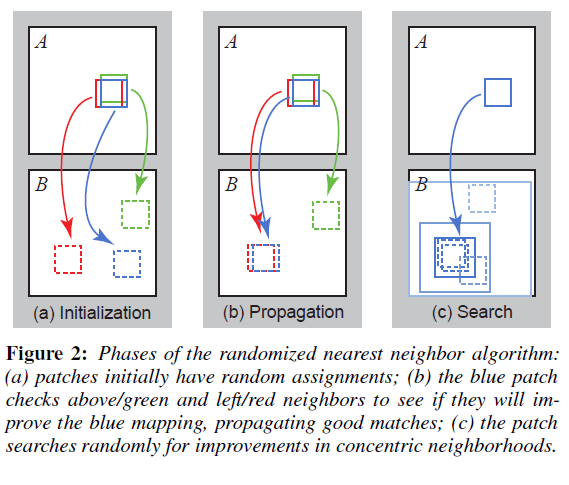
\includegraphics[scale=0.7]{pictures/fig1_patchmatch}
\end{frame}

\subsection{Computational Analysis}
\begin{frame}{Computational Analysis}
\begin{itemize}
\item Linear with respect to the image size
\item O(1) complexity of the binary representation
\end{itemize}
\end{frame}

\section{Evaluation}% To vanish after the other parts are done ! 
\subsection{Quantitative evaluation}
\begin{frame}{Quantitative evaluation}
\begin{itemize}
\item 2500 training images and 900 test images (500 articulated hand images and 400 interior images for 5 different environments)
\end{itemize}
\centering
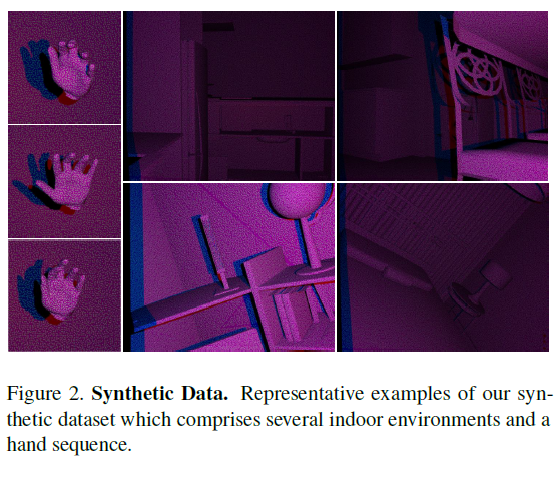
\includegraphics[scale=0.7]{pictures/fig2_synthetic_data}
\end{frame}

\subsection{Bias}
\begin{frame}{Bias}
\begin{itemize}
\item Average absolute depth error present in the whole set
\end{itemize}
\begin{figure}
\centering
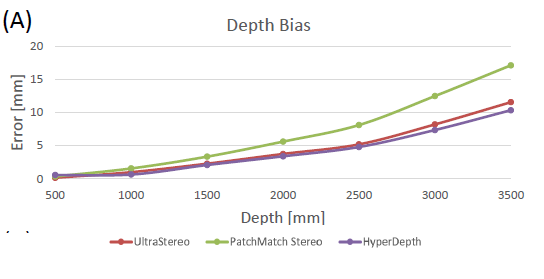
\includegraphics[scale=1]{pictures/fig3_depth_Bias_synthetic_data}
\caption{synthetic data}
\end{figure}
\end{frame}

\begin{frame}{Bias}
\begin{figure}
\centering
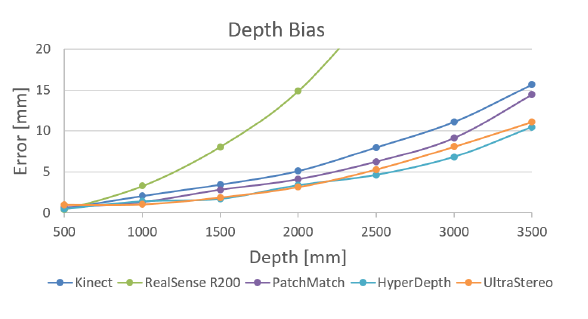
\includegraphics[scale=1]{pictures/fig_4_depth_bias_real_data}
\caption{real data}
\end{figure}
\end{frame}


